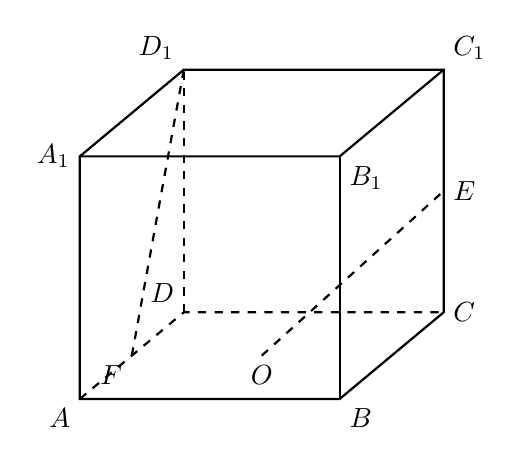
\begin{tikzpicture}[>=stealth, scale=1.1]
  % 顶点坐标
  \coordinate (A) at (0, 0);
  \coordinate (B) at (3.0, 0);
  \coordinate (C) at (4.2, 1.0);
  \coordinate (D) at (1.2, 1.0);

  \coordinate (A1) at (0, 2.8);
  \coordinate (B1) at (3.0, 2.8);
  \coordinate (C1) at (4.2, 3.8);
  \coordinate (D1) at (1.2, 3.8);

  % 中点坐标
  % O 为底面 ABCD 中心: (A+C)/2 = (2.1, 0.5)
  \coordinate (O) at (2.1, 0.5);
  % E 为 CC1 中点: (4.2, 2.4)
  \coordinate (E) at (4.2, 2.4);
  % F 为 AD 中点: (0.6, 0.5)
  \coordinate (F) at (0.6, 0.5);

  % 实线棱
  \draw[thick] (A) -- (B) -- (C) -- (C1) -- (D1) -- (A1) -- cycle;
  \draw[thick] (A1) -- (B1) -- (C1);
  \draw[thick] (B) -- (B1);

  % 虚线棱与辅助线
  \draw[dashed, thick] (A) -- (D) -- (C);
  \draw[dashed, thick] (D) -- (D1);

  % OE 和 FD1
  \draw[dashed, thick] (O) -- (E);
  \draw[dashed, thick] (F) -- (D1);

  % 节点标注
  \node[below left] at (A) {$A$};
  \node[below right] at (B) {$B$};
  \node[right] at (C) {$C$};
  \node[above left] at (D) {$D$};

  \node[left] at (A1) {$A_1$};
  \node[below right] at (B1) {$B_1$};
  \node[above right] at (C1) {$C_1$};
  \node[above left] at (D1) {$D_1$};

  \node[below] at (O) {$O$};
  \node[right] at (E) {$E$};
  \node[below left] at (F) {$F$};
\end{tikzpicture}
